
\chapter{集合}
\label{chap:set}

\section{文氏图}
\label{sec:venn-diagram}

\begin{example}
  一(4)班共有50人,其中28人有哥哥,26人有弟弟,15人没有兄弟。那么只有哥哥没有弟弟的有多少人?只有弟弟没有哥哥的有多少人?既有哥哥也有弟弟的有多少人?
\end{example}
\begin{proof}[提示]这种问题最适合用文氏图来解决。
  \begin{center}
    \begin{tikzpicture}[scale=1.0]
      \begin{scope}[blend mode=multiply]
        \draw(0,0)rectangle(4,3);
        \filldraw[fill=red!20,opacity=.5](1.5,1.5)circle(1);
        \filldraw[fill=blue!20,opacity=.5](2.5,1.5)circle(1);
        \draw[->](1,1.5)--(-.5,1.5)node[left]{有哥哥的};
        \draw[->](3,1.5)--(4.5,1.5)node[right]{有弟弟的};
        \draw[->](3.5,2.6)--(4,3.5)node[above]{没有兄弟的};
        \draw[->](2,1.5)--(0,3.5)node[above]{既有哥哥也有弟弟的};
      \end{scope}
    \end{tikzpicture}
  \end{center}
  如上图,用长方形表示整个班的人,左边的圆表示有哥哥的人,右边的圆表示有弟弟的人,两个圆相交的部分表示既有哥哥又有弟弟的人(如果班上没有既有哥哥也有弟弟的人,则两个圆不相交)。则左圆左边部分表示只有哥哥的人,右圆的右边部分表示只有弟弟的人,两圆外空白的部分表示没有兄弟的人。由此,可以先填入15。
  \begin{center}
    \begin{tikzpicture}[scale=1.0]
      \begin{scope}[blend mode=multiply]
        \draw(0,0)rectangle(4,3);
        \filldraw[fill=red!20,opacity=.5](1.5,1.5)circle(1);
        \filldraw[fill=blue!20,opacity=.5](2.5,1.5)circle(1);
        \node[above] at (3,0) {15};
      \end{scope}
      \begin{scope}[blend mode=multiply,shift={(4.5,0)}]
        \draw(0,0)rectangle(4,3);
        \filldraw[fill=red!20,opacity=.5](1.5,1.5)circle(1);
        \filldraw[fill=blue!20,opacity=.5](2.5,1.5)circle(1);
        \node[above] at (3,0) {15};
        \node at (2,1.5){19};
      \end{scope}
      \begin{scope}[blend mode=multiply,shift={(9,0)}]
        \draw(0,0)rectangle(4,3);
        \filldraw[fill=red!20,opacity=.5](1.5,1.5)circle(1);
        \filldraw[fill=blue!20,opacity=.5](2.5,1.5)circle(1);
        \node[above] at (3,0) {15};
        \node at (2,1.5){19};
        \node at (1.1,1.5){9};
        \node at (2.9,1.5){7};
      \end{scope}

      \draw[help lines,dashed,->](1.5,-.1)--(4.3,-2)node[color=black,midway,sloped,above]{方法2};

      \begin{scope}[blend mode=multiply,shift={(4.5,-4)}]
        \draw(0,0)rectangle(4,3);
        \filldraw[fill=red!20,opacity=.5](1.5,1.5)circle(1);
        \filldraw[fill=blue!20,opacity=.5](2.5,1.5)circle(1);
        \node[above] at (3,0) {15};
        %\node at (2,1.5){19};
        \node at (1.1,1.5){9};
        \node at (2.9,1.5){7};
      \end{scope}
      \begin{scope}[blend mode=multiply,shift={(9,-4)}]
        \draw(0,0)rectangle(4,3);
        \filldraw[fill=red!20,opacity=.5](1.5,1.5)circle(1);
        \filldraw[fill=blue!20,opacity=.5](2.5,1.5)circle(1);
        \node[above] at (3,0) {15};
        \node at (2,1.5){19};
        \node at (1.1,1.5){9};
        \node at (2.9,1.5){7};
      \end{scope}
    \end{tikzpicture}
  \end{center}
  两个圆加起来的部分共有$50-15=35$人,从而可以填入两圆共同的部分$28+26-35=19$人,只有哥哥的$28-19=9$人,只有弟弟的$26-19=7$人。

  另一种方法是知道两圆的和为35人后,左圆左半边为$35-26=9$人,右圆右半边为$35-28=7$人,中间为$28-9=19$人(或者$26-7=19$人)。
\end{proof}

\section{容斥原理}
\label{sec:inclusion-exclusion-principle}

\begin{definition}[计数]
  对任意集合$A$,用$|A|$表示集合中元素的个数。
\end{definition}

\begin{theorem}[容斥原理,Inclusion-Exclusion Principle]
  任意集合$A,B,C$,有
  \begin{align*}
    |A\cup B| ={}&       |A| + |B| - |A\cap B|\\
    |A\cup B\cup C| ={}& |A| + |B| + |C| - |A\cap B| - |B\cap C| - |C\cap A| + |A\cap B\cap C|
  \end{align*}
  更普遍的形式是,对任意集合$A_1,A_2,\cdots,A_n$,有
  \begin{align*}
    \left|\bigcup_{i=1}^n A_i\right| ={}& \sum_{i=1}^n\left|A_i\right|
    - \sum_{1\le i<j\le n}\left|A_i\cap A_j\right| + \sum_{1\le i<j<k\le n}\left|A_i\cap A_j\cap A_k\right| - \cdots\\
    & + (-1)^{n-1}\left|A_1\cap A_2\cap \cdots \cap A_n\right|
  \end{align*}
\end{theorem}
\begin{proof}[提示]用文氏图,可以直观地看出$n=2,3$时的情况。
  \begin{center}
    \begin{tikzpicture}[scale=1.0]
      \begin{scope}[blend mode=multiply]
        \filldraw[fill=red!20,opacity=.5](1.5,1.5)circle(1);
        \filldraw[fill=blue!20,opacity=.5](2.5,1.5)circle(1);
        \node at (1.1,1.5){$A$};
        \node at (2.9,1.5){$B$};
        \node[below] at (2,.3){$n=2$};
      \end{scope}
      \begin{scope}[blend mode=multiply,shift={(5,0)}]
        \filldraw[fill=red!20,opacity=.5](1.5,1.5)circle(1);
        \filldraw[fill=blue!20,opacity=.5](2.5,1.5)circle(1);
        \filldraw[fill=green!20,opacity=.5](2,2.5)circle(1);
        \node at ($(1.5,1.5)+(210:1.4)$){$A$};
        \node at ($(2.5,1.5)+(330:1.4)$){$B$};
        \node at ($(2,2.5)+(90:1.4)$){$C$};
        \node[below] at (2,.3){$n=3$};
        \foreach \x/\y/\v in{1.1/1.1/1, 2.9/1.1/2, 2/2.9/3,
          2/1.15/4, 1.375/2.1/6, 2.625/2.1/5, 2/1.9/7}{
          \node at(\x,\y){$S_{\v}$};
        }
      \end{scope}
    \end{tikzpicture}
  \end{center}
  如上图,当$n=2$时,$|A| + |B|$比$|A\cup B|$多加了一个$|A\cap B|$,所以有
  \begin{align*}
    |A\cup B| = |A| + |B| - |A\cap B|    
  \end{align*}
  当$n=3$时,如图将$A\cup B\cup C$分割成若干个不相交的部分,有
  \begin{align*}
    |A\cup B\cup C| ={}&
    %                    \left(A-(B\cup C)\right) \cup \left(B - (C\cup A)\right) \cup \left(C - (A\cup B)\right)\\
    % &\cup \left((A\cap B) - C\right) \cup \left((B\cap C) - A\right) \cup \left((C\cap A) - B\right)\\
    % &\cup (A\cap B\cap C)
        \left| S_1\cup S_2 \cup S_3 \cup S_4 \cup S_5 \cup S_6 \cup S_7 \right| \\
    ={}& \left| S_1 \right| + \left| S_2 \right| + \left| S_3 \right| + \left| S_4 \right| + \left| S_5 \right| + \left| S_6 \right| + \left| S_7 \right|
  \end{align*}
  再由图,可以直观地得到$S_i$与$A,B,C$之间的关系:
  \begin{align*}
    |A\cap B| ={}& |S_4\cup S_7| = |S_4| + |S_7|\\
    |B\cap C| ={}& |S_5\cup S_7| = |S_5| + |S_7|\\
    |C\cap A| ={}& |S_6\cup S_7| = |S_6| + |S_7|\\
    |A\cap B\cap C| ={}& |S_7|
  \end{align*}
  代入展开后可得。
\end{proof}

\section{极坐标}
\label{sec:polar-coordinate}

\begin{example}[极坐标的魔法]\mbox{}\par
  \begin{center}
    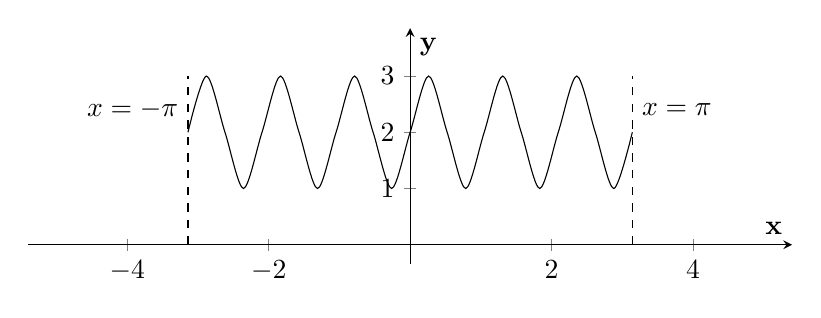
\begin{tikzpicture}[scale=1.0]
      % \draw[help lines](0,0)grid(4,3);
      \begin{axis}[anchor=origin,
      scale only axis,
      width=0.8\textwidth,
      height=3cm,
      xmin = -4.5,
      xmax = 4.5,
      ymin = 0,
      ymax = 3.5, 
      axis lines = middle,
      enlargelimits = true,
      xlabel = {$\mathbf{x}$},
      ylabel = {$\mathbf{y}$}% ,
      % yticklabels={,,},
      % xticklabels={,,}
      ]
      \coordinate (A) at (axis cs:40,6);
      \addplot[domain=-3.1415926:3.1415926,smooth] (\x, {sin(deg(6*\x)) + 2});
      \draw[dashed] (-3.1415926,0)--(-3.1415926,3)node[pos=.8,left]{$x=-\pi$};
      \draw[dashed] (3.1415926,0)--(3.1415926,3)node[pos=.8,right]{$x=\pi$};
    \end{axis}
    \end{tikzpicture}
  \end{center}
  上面曲线在直角坐标系下的函数表达式为
  \begin{align*}
    y = \sin(6x) + 2
  \end{align*}
  相像一下,把$x$轴以及$x=-\pi$和$x=\pi$两直线围成的区域弯成一个圆,会是什么样呢?即将上面的函数变为极坐标形式
  \begin{align*}
    r = \sin(6\theta) + 2
  \end{align*}
  \begin{center}
    \begin{tikzpicture}[scale=1.0]
      \begin{polaraxis}
        \addplot+[mark=none,domain=0:360,samples=600]{sin(6*x)+2};
      \end{polaraxis}
    \end{tikzpicture}
  \end{center}
  这就是极坐标的魔力。
\end{example}

\begin{example}
  考虑曲线
  \begin{align*}
    y = \sin(2x) \cos(2x)
  \end{align*}
  \begin{center}
    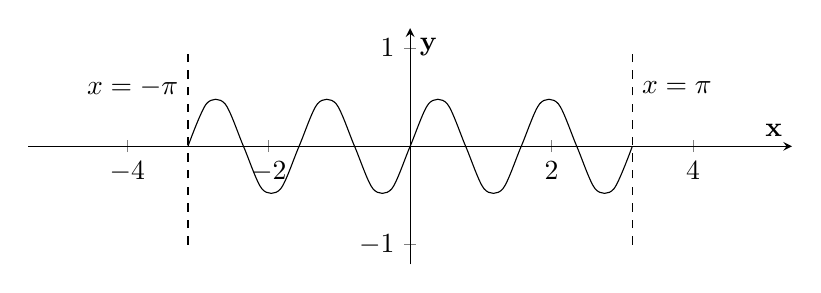
\begin{tikzpicture}[scale=1.0]
      % \draw[help lines](0,0)grid(4,3);
      \begin{axis}[anchor=origin,
      scale only axis,
      width=0.8\textwidth,
      height=3cm,
      xmin = -4.5,
      xmax = 4.5,
      ymin = -1,
      ymax = 1, 
      axis lines = middle,
      enlargelimits = true,
      xlabel = {$\mathbf{x}$},
      ylabel = {$\mathbf{y}$}% ,
      % yticklabels={,,},
      % xticklabels={,,}
      ]
      \coordinate (A) at (axis cs:40,6);
      \addplot[domain=-3.1415926:3.1415926,smooth] (\x, {sin(deg(2*\x)) * cos(deg(2*x))});
      \draw[dashed] (-3.1415926,-1)--(-3.1415926,1)node[pos=.8,left]{$x=-\pi$};
      \draw[dashed] (3.1415926,-1)--(3.1415926,1)node[pos=.8,right]{$x=\pi$};
    \end{axis}
    \end{tikzpicture}
  \end{center}
  弯成圆时,曲线变为
  \begin{align*}
    r = \sin(2\theta)\cos(2\theta)
  \end{align*}
    \begin{center}
    \begin{tikzpicture}[scale=1.0]
      \begin{polaraxis}
        \addplot+[mark=none,domain=0:360,samples=600]{sin(2*x)*cos(2*x)};
      \end{polaraxis}
    \end{tikzpicture}
  \end{center}
\end{example}